% Copyright (c) 2015 William Bevington, Callum O'Brien and Alex Pace

% Permission is granted to copy, distribute and/or modify this document
% under the terms of the GNU Free Documentation License, Version 1.3
% or any later version published by the Free Software Foundation;
% with no Invariant Sections, no Front-Cover Texts, and no Back-Cover Texts.

\documentclass{article}

\usepackage{amsmath}
\usepackage{amssymb}

\usepackage{tikz}

\usepackage{geometry}

\title{Edexcel Advanced Level GCE Mathematics FP1}
\author{William Bevington \and Callum O'Brien \and Alex Pace}
\date{}

\begin{document}

\maketitle
\tableofcontents
\newpage

\section{Matrices}
A matrix is a grid of values:

\[\left(\begin{array}{cc} a & b \\ c & d \end{array}\right)\]

similar matrices can be added with each term adding to the corresponding term on the other matrix. Multlipication however is a little more complex. The first matrix must have the same number of columns as the second matrix has rows. This is because when you muliply a matrix by another, you take the top row of the first and times each number by it's partner in the frist column of the second, this give you your value for the top left corner of your new matrix. e.g.

\[\left(\begin{array}{ccc} 1 & 2 & 3 \\ 5 & 10 & -1 \end{array}\right) \times \left(\begin{array}{cc} 0 & 2 \\ 3 & -1 \\ 1 & 0 \end{array}\right) = \left(\begin{array}{cc} 9 & 0 \\ 29 & 0 \end{array}\right)\]

Matrices can also be used to solve simultaneous equations using a matrix (\(m\)) and it's inverse (\(m^{-1})\). (\(m^{-1})\) can be found through the following process:

\[m=\left(\begin{array}{cc} a & b \\ c & d \end{array}\right) \therefore m^{-1} = \frac{1}{ad-bc}\left(\begin{array}{cc} d & -b \\ -c & a \end{array}\right)\]

The denominator of the fraction above is known as the ``determinate". The following example walks through solving a simultaneous equation using matrices:

\[3x+5y=1\]
\[7x-2y=16\]

This can be rearanged into the following:

\[\left(\begin{array}{cc} 3 & 5 \\ 7 & -2 \end{array}\right)\left(\begin{array}{c} x \\ y \end{array}\right)=\left(\begin{array}{c} 1 \\ 16 \end{array}\right)\]
\[m=\left(\begin{array}{cc} 3 & 5 \\ 7 & -2 \end{array}\right) \hspace{0.5cm} \text{\textit{determinate of} } m=\left(-6-35\right)=-41\]
\[ \therefore m^{-1} = \frac{1}{-41} \left(\begin{array}{cc} -2 & -5 \\ -7 & 3 \end{array}\right)\]

Multiplying both sides of our matrix equation by the inverse of \(m\) results in the following:

\[\left(\begin{array}{c} x \\ y \end{array}\right) = \frac{1}{-41} \left(\begin{array}{cc} -2 & -5 \\ -7 & 3 \end{array}\right) \left(\begin{array}{c} 1 \\ 16 \end{array}\right)\]
\[\left(\begin{array}{c} x \\ y \end{array}\right) = \frac{1}{-41} \left(\begin{array}{c} -82 \\ 41 \end{array}\right)\]
\[x=2 \hspace{0.3cm} \& \hspace{0.2cm} y=-1\]

\subsection{Matrix Transformations}

It makes things easy to imagine that a transformation matrix maps the unit square of the transformed plane, which is why the identity matrix, below,  has no effect, it maps the corners of our unit square to the same place.

\[\left(\begin{array}{cc} 1 & 0 \\ 0 & 1 \end{array}\right)\]

And this is an example of a transformation matrix that rotates the axis \(\frac{\pi}{2}\) anticlockwise:

\[\left(\begin{array}{cc} 0 & -1 \\ 1 & 0 \end{array}\right)\]

The determinate of a transformation matrix is its area scale factor. \\ but what if one wants to rotate a matrix through any arbitrary angle, the general rotation matrix, below, rotates a matrix through any angle \(\theta\) clockwise.

\[\left(\begin{array}{cc} \cos\left(\theta\right) & -\sin\left(\theta\right) \\ \sin\left(\theta\right) & \cos\left(\theta\right) \end{array}\right)\]

When combining Matrix transformations, they occur in reverse order. for example, applying transformation matrices \(A\) and \(B\) to matrix \(m\) in the order \(ABm\) applyies the transformations \(B\), followed by \(A\).

\section{Inverse Matrix Transformations}

if \(A\) is a transformation matrix then the inverse of \(A\);\(A^{-1}\) will be the opposite transformation and return to the original shape.

\[AA^{-1}=I\]
\[\text{If \(A\) \(=\) }\left(\begin{array}{cc} a & b \\ c & d \end{array}\right) \text{  Then \(A^{-1}\) \(=\) } \frac{1}{ad-bc}\left(\begin{array}{cc} d & -b \\ -c & a \end{array}\right)\]
\[detA=ad-bc\]

If a shape has area \(X\) then after the transformation \(A\), the area is \(X \times |detA|\). \\

If \(detA\) is zero then \(A\) is said to be singular, and \(A^{-1}\) does not exist:

\[\text{\(A\) non-singular } \leftrightarrow detA\neq 0 \leftrightarrow A^{-1} \text{ exists.}\]

\textbf{Prove that} \(\left(PQ\right)^{-1}\) \(=\) \(Q^{-1}P^{-1}\)
\[AA^{-1}=I \hspace{0.2cm} \therefore \hspace{0.2cm} \left(PQ\right)\left(PQ\right)^{-1}=I\]
\[PQ\left(PQ\right)^{-1}=I\]
\[P^{-1}PQ\left(PQ\right)^{-1}=P^{-1}I \hspace{0.2cm} \rightarrow \hspace{0.2cm} IQ\left(PQ\right)^{-1}=P^{-1}\]
\[\therefore \hspace{0.2ccm} Q\left(PQ\right)^{-1}=P^{-1}\]
\[Q^{-1}Q\left(QP\right)^{-1}=Q^{-1}P^{-1} \hspace{0.2cm} \rightarrow \hspace{0.2cm} I\left(PQ\right)^{-1}=Q^{-1}P^{-1}\]
\[\therefore \hspace{0.2cm} \left(PQ\right)^{-1}=Q^{-1}P^{-1}\]

\section{Complex Numbers}

If the complex numbers \(z_1\) and \(z_2\) are equal, then it follows that \(Re\left(z_1\right) = Re\left(z_2\right)\) and \(Im\left(z_1\right) = Im\left(z_2\right)\). as demonstrated:

\paragraph{Let} \(z_1 = a+bi\) and \(z_2 = c+di\) where \(a,b,c,d, \in \mathbb{R}\)

\[z_1 = z_2 \therefore a+bi = c+di\]
\[a-c=\left(d-b\right)i\]
\[\left(a-c\right)^2=\left(b-d\right)^2i^2 \rightarrow \left(a-c\right)^2=-\left(d-b\right)^2\]
\[\left(a-c\right)^2\geq 0 \& -\left(d-b\right)^2\leq 0\]

\noindent The only overlap here is 0, so \(Re\left(z_1\right) = Im\left(z_2\right)\)

\subsection{Modulus \& Argument of Complex Numbers}

These values are given when a complex number is represented in the polar form:
\[z=r\left(\cos\left(\theta\right) + i\sin\left(\theta\right)\right)\]
where \(r\) is the modulus and \(\theta\) is the argument. From the cartesian form \(z=a+bi\) the modulus and argument of a complex number can be found as follows:

\[|z|=\sqrt{a^2 + b^2}\]
\[arg\left(z\right) = arctan\left(\frac{b}{a}\right)\]

\subsection{Exponential form of Complex Numbers}

Let \(z\) be a complex number such that \(z=\cos\left(\theta\right) +i\sin\left(\theta\right)\), it follows that, through differentiating:

\[\frac{dz}{d\theta}=-\sin\left(\theta\right) +i\cos\left(\theta\right)\]

\noindent It can then be said that \(z\) is a multiple of \(\frac{dz}{d\theta}\), and by definition the only function that can be a multiple of itself after differentiation is the natural exponent \(e\), so it must follow that:

\[e^{i\theta}=\cos\left(\theta\right) +i\sin\left(\theta\right)\]

\noindent Adding the modulus we get:

\[re^{i\theta} = r(\cos\left(\theta\right) +i\sin\left(\theta\right))\]

\noindent Using this definition it is possible to describe the \(\sin\) and \(\cos\) functions by using the following equations:

\[e^{i\theta}= \cos\left(\theta\right)+i\sin\left(\theta\right)\]
\[e^{-i\theta}=\cos\left(\theta\right)-i\sin\left(\theta\right)\]

\noindent Therefore:

\[e^{i\theta}+e^{-i\theta}=2\cos\left(\theta\right)\]
\[\frac{e^{i\theta}+e^{-i\theta}}{2}=\cos\left(\theta\right)\] \\\\

Similarly:

\[\frac{e^{i\theta}-e^{-i\theta}}{2i}=\sin\left(\theta\right)\]

\section{Conic Sections}

\begin{center}
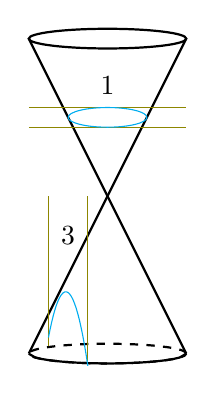
\begin{tikzpicture}[xscale=0.5,yscale=0.5]
    \draw[thick, domain=-2:2] plot (\x, {2*\x});
    \draw[thick, domain=-2:2] plot (\x, {-2*\x});
    \draw[thick] (0,4) ellipse (2 and 1/4);
    \draw[thick, domain=2:-2] plot (\x, {0.125*(-sqrt(4-(\x*\x))-32)});
    \draw[thick, dashed] (0,-4) ellipse (2 and 1/4);
    \draw[olive] (-2,1.75) -- (2,1.75);
    \draw[olive] (-2,2.25) -- (2,2.25);
    \draw[cyan] (0,2) ellipse (1 and 1/4);
    \node at (0,2.8) {1};
    \draw[olive] (-1.5,-3.8) -- (-1.5,0);
    \draw[olive] (-0.5,-4.2) -- (-0.5,0);
    \draw[cyan, domain=-1.5:-0.5] plot (\x, {-6*((\x+1.06)*(\x+1.06))-2.43});
    \node at (-1,-1) {3};
\end{tikzpicture} \hspace{50pt} 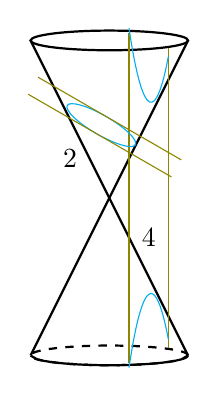
\begin{tikzpicture}[xscale=0.5,yscale=0.5]
    \draw[thick, domain=-2:2] plot (\x, {2*\x});
    \draw[thick, domain=-2:2] plot (\x, {-2*\x});
    \draw[thick] (0,4) ellipse (2 and 1/4);
    \draw[thick, domain=2:-2] plot (\x, {0.125*(-sqrt(4-(\x*\x))-32)});
    \draw[thick, dashed] (0,-4) ellipse (2 and 1/4);
    \draw[olive] (1.5,-3.8) -- (1.5,3.8);
    \draw[olive] (0.5,-4.2) -- (0.5,4.2);
    \draw[cyan, domain=1.5:0.5] plot (\x, {-6*((\x-1.06)*(\x-1.06))-2.43});
    \draw[cyan, domain=1.5:0.5] plot (\x, {6*((\x-1.06)*(\x-1.06))+2.43});
    \node at (1,-1) {4};
    \draw[cyan, rotate=330] (-1.1,1.5) ellipse (1 and 1/4);
    \draw[olive, rotate=330] (-3.1,1.75) -- (1.1,1.75);
    \draw[olive, rotate=330] (-3.1,1.25) -- (1.1,1.25);
    \node at (-1,1) {2};
\end{tikzpicture}
\end{center}

\begin{center}
\begin{tabular}{cccc}
    1. Circle & 2. Ellipse & 3. Parabola & 4. Hyperbola \\
\end{tabular}
\end{center}

\noindent The shapes specified above are known as conic sections as they can be constructed using cross sections of cones.

\subsection{Parabolas}

The general parametric equation of a parabola:

\[y=2at\]
\[x=at^2\]

\noindent It follows then, that the general cartesian equation of a parabola is:

\[y^2=4ax\]

\noindent The constant, \(a\), of a parabola is of quite some significance. The Focus of the parabola can be described as the point on the x axis who's distance from any point on the parabola is the same as the horizontal distance from that point on the curve and the directrix of a parabola. The focus of a parabola possesses the coordinates \((a,0)\), and the directrix of a parabola is described by the line \(x=-a\). The diagram below illustrates this.

\begin{center}
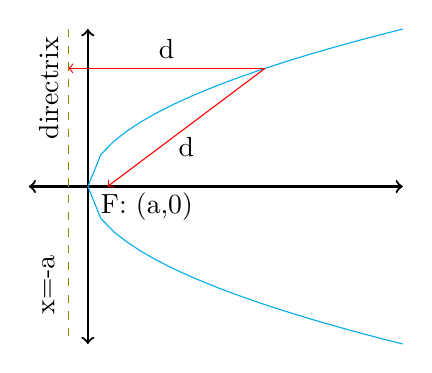
\begin{tikzpicture}[xscale=0.25, yscale=0.25]
    \draw[thick, <->] (0,8) -- (0,-8);
    \draw[thick, <->] (-3,0) -- (16,0);
    \draw[olive, dashed] (-1,8) -- (-1,-8);
    \draw[cyan, domain=0:16] plot (\x, {2*sqrt(\x)});
    \draw[cyan, domain=0:16] plot (\x, {-2*sqrt(\x)});
    \draw[red, <-] (-1,6) -- (9,6);
    \draw[red, ->] (9,6) -- (1,0);
    \node at (4,7) {d};
    \node at (5,2) {d};
    \node at (3,-1) {F: (a,0)};
    \node[rotate=90] at (-2,5) {directrix};
    \node[rotate=90] at (-2,-5) {x=-a};
\end{tikzpicture}
\end{center}

\noindent The concept of the focus and directrix can be proved through the following process:\\

\noindent General point \(p\) on the curve:

\[p(x,y) \:=\: p\left(at^2,2at\right)\]

\noindent consider a point \(D\) on the directrix, and \(P\) on the curve in the same horizontal plane as \(D\):

\[D\rightarrow P \:=\: a+at^2\]
\[P\rightarrow F \:=\: \sqrt{\left(at^2-a\right)^2+\left(2at\right)^2} \:=\: \sqrt{a^2t^4-2a^2t^2+a^2=4a^2t^2}\]
\[\rightarrow\: \sqrt{a^2t^4+2a^2t^2+a^2} \:\rightarrow\: \sqrt{\left(a+at^2\right)^2}\]
\[\therefore \: P\rightarrow F \:=\: a+at^2\]
\[\therefore \: P\rightarrow F \:=\: D\rightarrow P\]

\end{document}

